\themaA
\graphicspath{{../../S03_En_route_vers_la_programmation/Images/}}

% Grille
\newcommand{\cn}{\psframe[fillstyle=solid,fillcolor=black](0,0)(1,1)}
\newcommand{\ho}{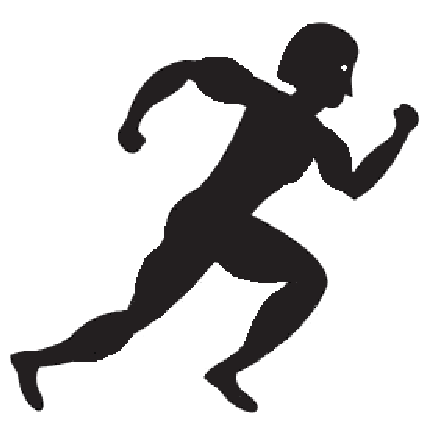
\includegraphics[width=0.3cm]{Hercule}}
\newcommand{\po}{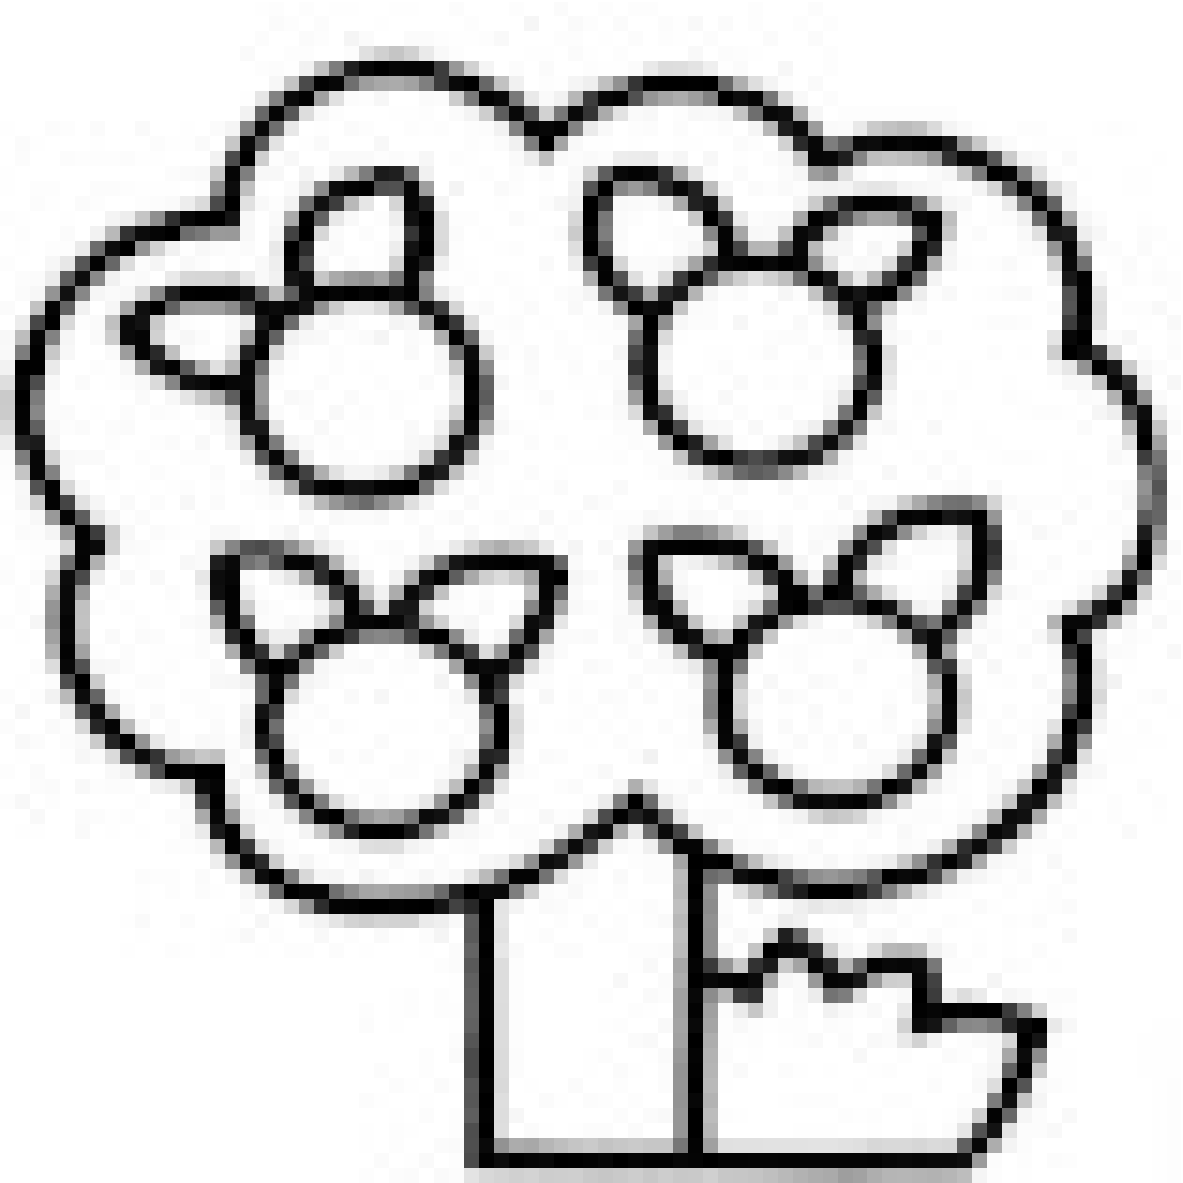
\includegraphics[width=0.3cm]{pommier}}

% Commandes
\newcommand{\dep}{\pspolygon[fillstyle=solid,fillcolor=orange](6,1)(0,1)(0,0)(1,0)(1.25,-0.25)(1.5,0)(6.5,0)(6.5,0.5) \pswedge[fillstyle=solid,fillcolor=orange,linecolor=orange](6,0.5){0.5}{0}{90} \psarc(6,0.5){0.5}{0}{90} \put(0.5,0.3){\footnotesize Démarre}}
\newcommand{\av}[1]{\pspolygon[fillstyle=solid,fillcolor=green](0,0)(1,0)(1.25,-0.25)(1.5,0)(6.5,0)(6.5,1)(1.5,1)(1.25,0.75)(1,1)(0,1) \put(0.5,0.3){\footnotesize Avance de #1}}
\newcommand{\tg}{\pspolygon[fillstyle=solid,fillcolor=yellow](0,0)(1,0)(1.25,-0.25)(1.5,0)(6.5,0)(6.5,1)(1.5,1)(1.25,0.75)(1,1)(0,1) \put(0.5,0.3){\footnotesize Tourne à gauche}}
\newcommand{\td}{\pspolygon[fillstyle=solid,fillcolor=pink](0,0)(1,0)(1.25,-0.25)(1.5,0)(6.5,0)(6.5,1)(1.5,1)(1.25,0.75)(1,1)(0,1) \put(0.5,0.3){\footnotesize Tourne à droite}}
\newcommand{\fin}{\pspolygon[fillstyle=solid,fillcolor=orange](0,0)(6,0)(6.5,0.5)(6.5,1)(1.5,1)(1.25,0.75)(1,1)(0,1)(0,0) \pswedge[fillstyle=solid,fillcolor=orange,linecolor=orange](6,0.5){0.5}{-90}{0} \psarc(6,0.5){0.5}{-90}{0} \put(0.5,0.3){\footnotesize Prends les pommes}}

% Fourmi
\newcommand{\fourmi}[3]{\rput{#3}(#1,#2){\psdot[linecolor=red,dotstyle=triangle*,linewidth=1mm](0,0)}}
\newcommand{\cub}{\psframe[fillstyle=solid,fillcolor=black](0,0)(1,1)}

\chapter{En route vers la\\programmation}
\label{S03}


%%%%%%%%%%%%%%%%%%%%%%%%%%%%%%%%
%%%%%%%%%%%%%%%%%%%%%%%%%%%%%%%%
\begin{autoeval}
   \small
   Niveau 1 (possibilité d'aller au delà).
   \begin{enumerate}
      \item Il réalise des activités d’algorithmique débranchée.
      \item Il met en ordre et/ou complète des blocs fournis par le professeur pour construire un programme simple sur un logiciel de programmation.
      \item Il écrit un script de déplacement ou de construction géométrique utilisant des instructions conditionnelles et/ou la boucle \og Répéter \dots{} fois \fg.
   \end{enumerate}
\end{autoeval}

\begin{prerequis}
   \begin{itemize}
      \item Notions d'algorithme et de programme. 
      \item Notion de variable informatique.
      \item Déclenchement d'une action par un événement.
      \item Séquences d'instructions, boucles, instructions conditionnelles.
      \item[\com] Écrire, mettre au point (tester, corriger) et exécuter un programme en réponse à un problème donné.
   \end{itemize}
\end{prerequis}

\vfill

\begin{debat}[Débat : la fourmi de Langton : que se passe-t-il ensuite ?] 
   La {\bf fourmi de Langton}, du nom de son inventeur scientifique américain {\it Christopher Langton}, est un petit programme informatique inventé vers la fin des années 1980. Il consiste en un automate qui se déplace dans un quadrillage suivant des règles simples. Il modélise le fait qu'un ensemble de comportements élémentaires peut donner lieu à un comportement complexe.
   \begin{center}
      {\psset{unit=0.2}
      \begin{pspicture}(0,0)(13,13)
         \fourmi{6.5}{6.5}{-90}
         \rput(2,0){\cub} \rput(3,0){\cub}
         \rput(1,1){\cub} \rput(2,1){\cub} \rput(9,1){\cub} \rput(10,1){\cub}
         \rput(0,2){\cub} \rput(2,2){\cub} \rput(3,2){\cub} \rput(5,2){\cub} \rput(8,2){\cub} \rput(11,2){\cub}
         \rput(0,3){\cub} \rput(3,3){\cub} \rput(5,3){\cub} \rput(6,3){\cub} \rput(7,3){\cub} \rput(9,3){\cub} \rput(10,3){\cub} \rput(11,3){\cub}
         \rput(1,4){\cub} \rput(3,4){\cub} \rput(10,4){\cub} \rput(12,4){\cub}
         \rput(3,5){\cub} \rput(4,5){\cub} \rput(8,5){\cub} \rput(9,5){\cub}
         \rput(3,6){\cub} \rput(4,6){\cub} \rput(5,6){\cub} \rput(7,6){\cub} \rput(8,6){\cub} \rput(9,6){\cub}
         \rput(3,7){\cub} \rput(4,7){\cub} \rput(8,7){\cub} \rput(9,7){\cub}
         \rput(0,8){\cub} \rput(2,8){\cub} \rput(9,8){\cub} \rput(11,8){\cub}
         \rput(0,9){\cub} \rput(1,9){\cub} \rput(2,9){\cub} \rput(5,9){\cub} \rput(6,9){\cub} \rput(7,9){\cub} \rput(9,9){\cub} \rput(12,9){\cub}
         \rput(1,10){\cub} \rput(4,10){\cub} \rput(7,10){\cub} \rput(9,10){\cub} \rput(10,10){\cub} \rput(12,10){\cub}
         \rput(2,11){\cub} \rput(3,11){\cub} \rput(10,11){\cub} \rput(11,11){\cub}
         \rput(9,12){\cub} \rput(10,12){\cub}
      \end{pspicture}}
   \end{center}
   \bigskip
   \begin{cadre}[B2][J4]
      \begin{center}
         Vidéo : \href{https://www.youtube.com/watch?v=qZRYGxF6D3w}{\bf La fourmi de Langton}, chaîne YouTube {\it Science étonnante}.
      \end{center}
   \end{cadre}
\end{debat}


%%%%%%%%%%%%%%%%%%%%%%%%%%%%%%%%%%%
%%%%%%%%%%%%%%%%%%%%%%%%%%%%%%%%%%%
\activites

\begin{activite}[La fourmi de Langton]
   {\bf Objectifs :} suivre un algorithme de déplacement ; se repérer dans le plan dans un repérage relatif.
   \begin{QCM}
      La fourmi de Langton est un automate qui se déplace dans un quadrillage suivant les règles suivantes :
      \begin{itemize}
         \item au départ, toutes les cases sont de la même couleur, ici blanches ;
         \item si la fourmi est sur une case blanche, elle tourne de \udeg{90} vers la droite, change la couleur de la case en noir et avance d'une case ;
         \item si la fourmi est sur une case noire, elle tourne de \udeg{90} vers la gauche, change la couleur de la case en blanc et avance d'une case.
      \end{itemize}
      Compléter dans les quadrillages ci-dessous les quinze premières étapes du déplacement de la fourni.
      \begin{center}
      \psset{unit=0.5,subgriddiv=1,gridlabels=0mm,gridcolor=gray}
      \small
      \begin{pspicture}(0,-0.7)(7,7)
         \psgrid(0,0)(7,7)
         \fourmi{3.5}{3.5}{0}
          \rput(3.5,-0.5){étape 0}
      \end{pspicture}
      \quad
      \begin{pspicture}(0,-0.7)(7,7)
         \psframe[fillstyle=solid,fillcolor=darkgray](3,3)(4,4)
         \psgrid(0,0)(7,7)
         \fourmi{4.5}{3.5}{-90}
         \rput(3.5,-0.5){étape 1}
      \end{pspicture}
      \quad
      \begin{pspicture}(0,-0.7)(7,7)  
         \psframe[fillstyle=solid,fillcolor=darkgray](3,3)(5,4)
         \psgrid(0,0)(7,7)
         \fourmi{4.5}{2.5}{180}
         \rput(3.5,-0.5){étape 2}
      \end{pspicture}
      \quad
      \begin{pspicture}(0,-0.7)(7,7)
         \psgrid(0,0)(7,7)
         \rput(3.5,-0.5){étape 3}
      \end{pspicture}
      \bigskip
      \begin{pspicture}(0,-0.7)(7,7)
         \psframe[fillstyle=solid,fillcolor=darkgray](3,2)(5,4)
         \psgrid(0,0)(7,7)
         \fourmi{3.5}{3.5}{0}
         \rput(3.5,-0.5){étape 4}
      \end{pspicture}
      \quad
      \begin{pspicture}(0,-0.7)(7,7)
         \psgrid(0,0)(7,7)
         \rput(3.5,-0.5){étape 5}
      \end{pspicture}
      \quad
      \begin{pspicture}(0,-0.7)(7,7)
         \psgrid(0,0)(7,7)
         \rput(3.5,-0.5){étape 6}
      \end{pspicture}
      \quad
      \begin{pspicture}(0,-0.7)(7,7)
         \psframe[fillstyle=solid,fillcolor=darkgray](2,3)(3,5)
         \pspolygon[fillstyle=solid,fillcolor=darkgray](3,2)(5,2)(5,4)(4,4)(4,3)(3,3)
         \psgrid(0,0)(7,7)
         \fourmi{3.5}{4.5}{-90}
         \rput(3.5,-0.5){étape 7}
      \end{pspicture}
      \bigskip
      \begin{pspicture}(0,-0.7)(7,7)
         \psgrid(0,0)(7,7)
         \rput(3.5,-0.5){étape 8}
      \end{pspicture}
      \quad
      \begin{pspicture}(0,-0.7)(7,7)
         \psgrid(0,0)(7,7)
         \rput(3.5,-0.5){étape 9}
      \end{pspicture}
      \quad
      \begin{pspicture}(0,-0.7)(7,7)
         \psgrid(0,0)(7,7)
         \rput(3.5,-0.5){étape 10}
      \end{pspicture}
      \quad
      \begin{pspicture}(0,-0.7)(7,7)
         \pspolygon[fillstyle=solid,fillcolor=darkgray](2,2)(5,2)(5,4)(4,4)(4,5)(2,5)(2,4)(3,4)(3,3)(2,3)
         \psgrid(0,0)(7,7)
         \rput(3.5,-0.5){étape 11}
         \fourmi{1.5}{2.5}{90}
      \end{pspicture}
      \bigskip
      \begin{pspicture}(0,0)(7,7)
         \psgrid(0,0)(7,7)
         \rput(3.5,-0.5){étape 12}
      \end{pspicture}
      \quad
      \begin{pspicture}(0,0)(7,7)
         \psgrid(0,0)(7,7)
         \rput(3.5,-0.5){étape 13}
      \end{pspicture}
      \quad
      \begin{pspicture}(0,0)(7,7)
         \psgrid(0,0)(7,7)
         \rput(3.5,-0.5){étape 14}
      \end{pspicture}
      \quad
      \begin{pspicture}(0,0)(7,7)
         \psgrid(0,0)(7,7)
         \rput(3.5,-0.5){étape 15}
      \end{pspicture} 
      \end{center}
   \end{QCM}
\end{activite}


%%%%%%%%%%%%%%%%%%%%%%%%%%%%%%%%%%
%%%%%%%%%%%%%%%%%%%%%%%%%%%%%%%%%%
\cours 

%%%%%%%%%%%%%%%%%%%%%%%%%%
\section{Algorithmes et langages de programmation}

\begin{definition}[Algorithme]
   Un {\bf algorithme} est une liste ordonnée et logique d'instructions permettant de réaliser une tâche de manière automatisée.
\end{definition}

\medskip
 
Un algorithme peut-être traduit, grâce à un langage de programmation, en un programme exécutable par un ordinateur. Ce langage peut être formel, textuel, visuel\dots{} Actuellement, le logiciel utilisé au collège est Scratch, développé par le MIT. Les programmes sont créés grâce à une succession de blocs, chacun ayant une fonction.
\begin{center}
   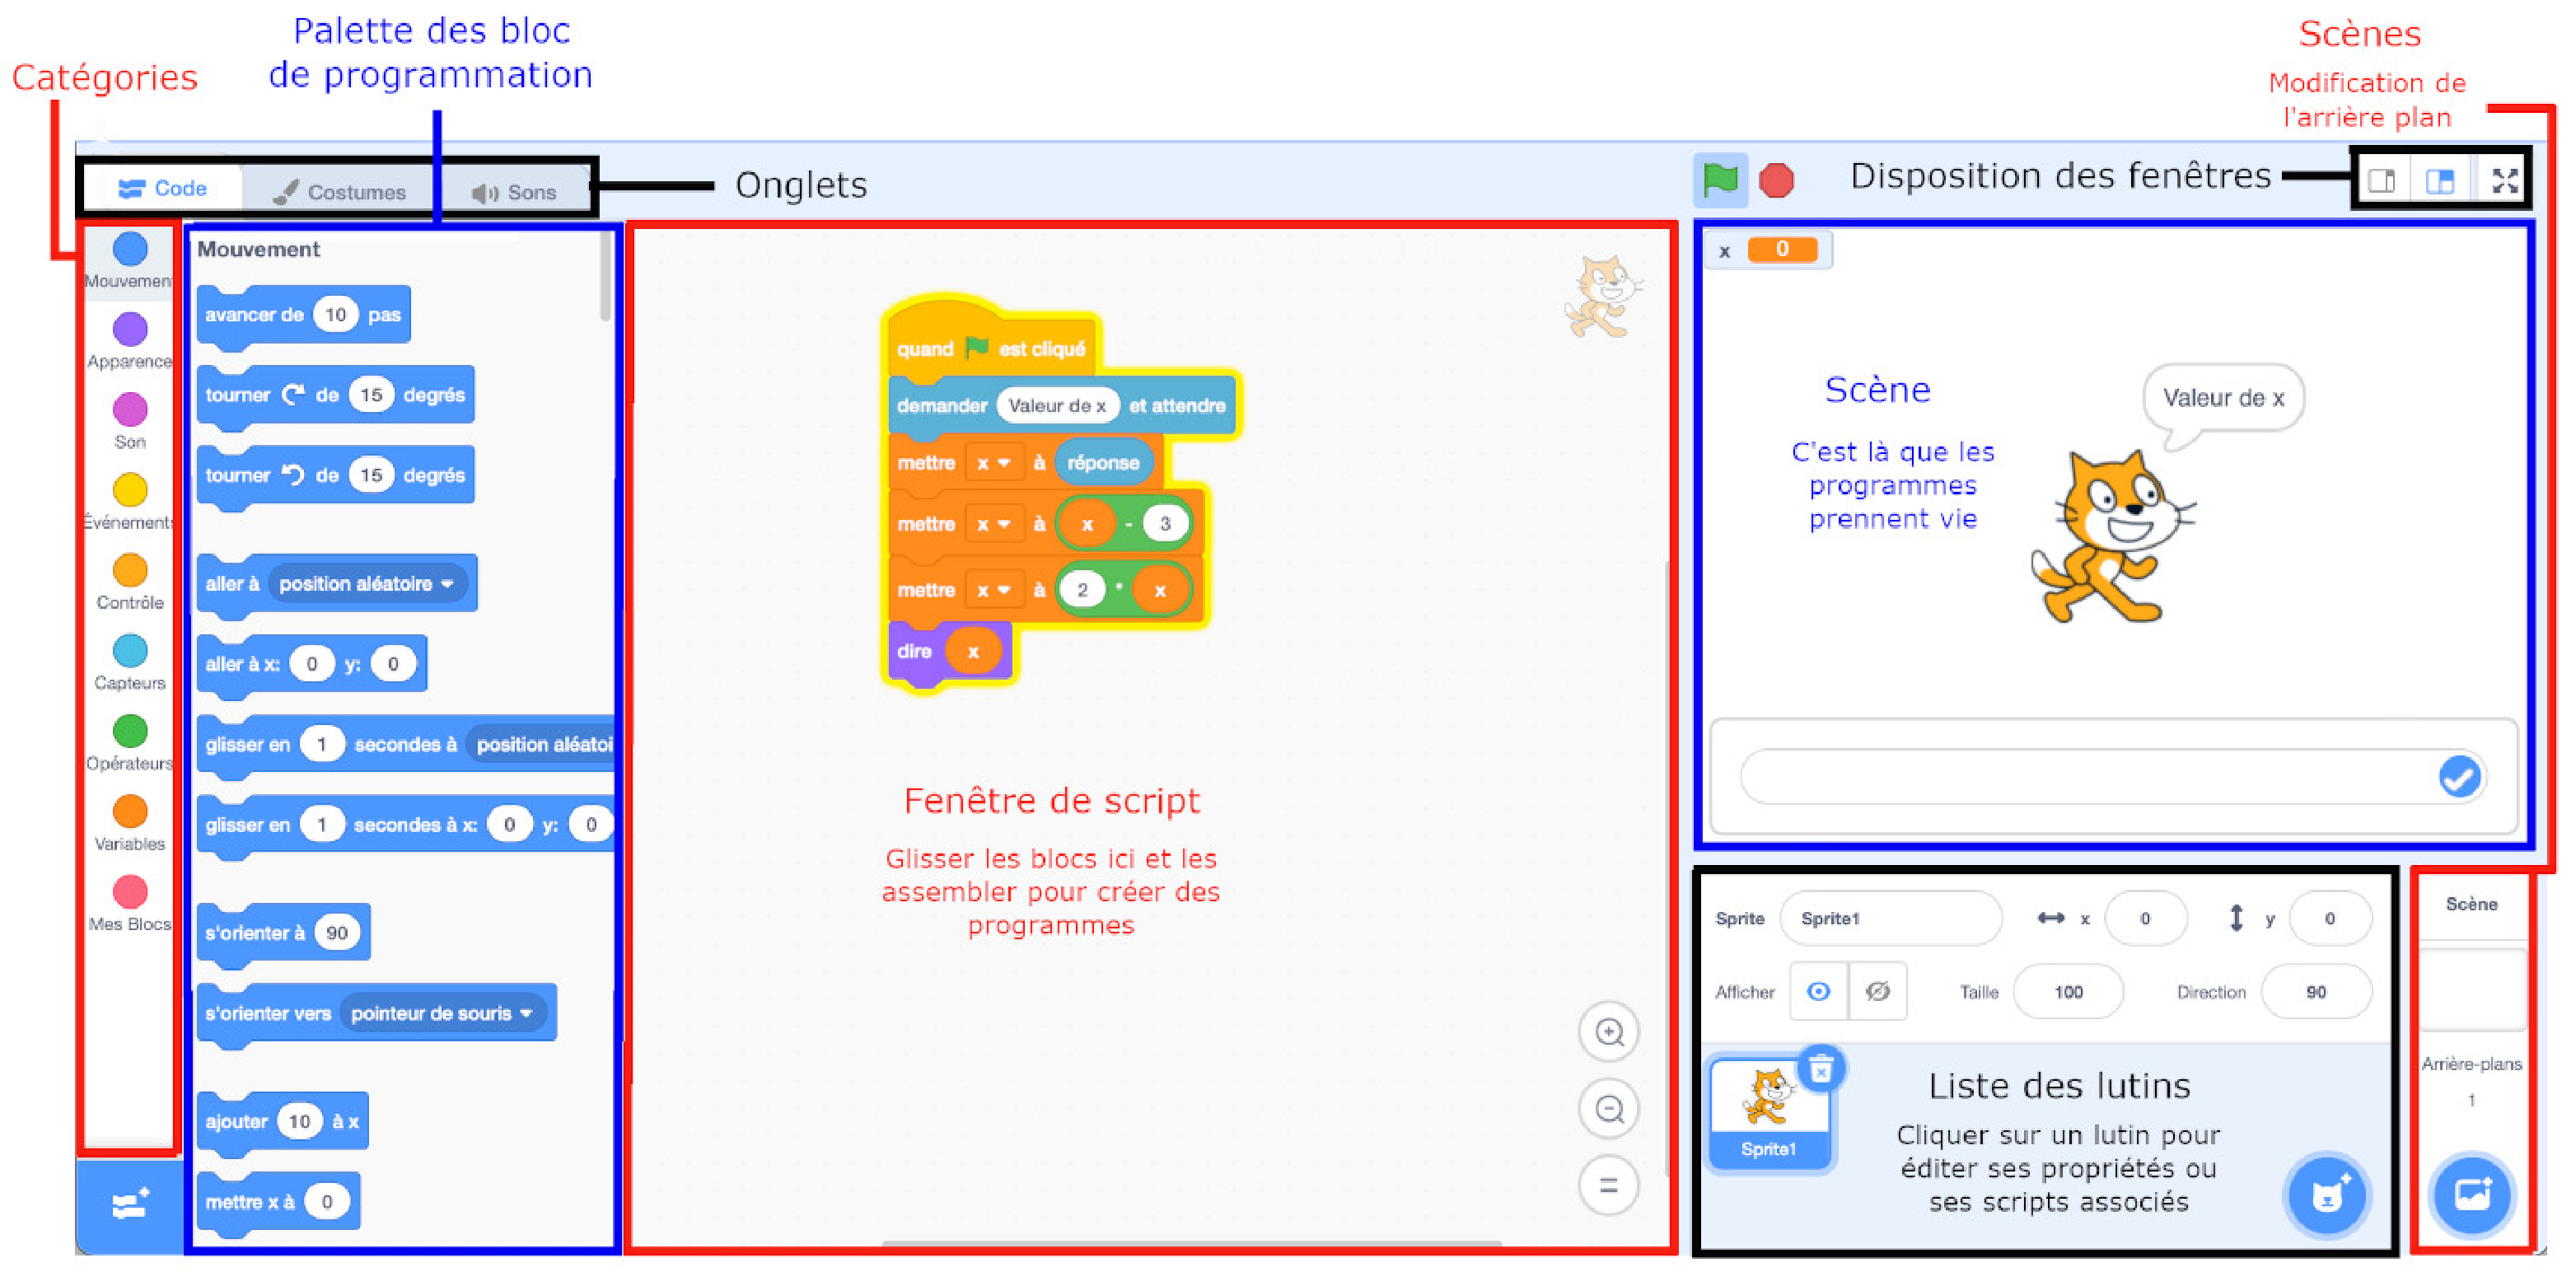
\includegraphics[width=16cm]{Interface_Scratch}
\end{center}


%%%%%%%%%%%
\section{Se déplacer}

\begin{methode}[Langages de déplacement]
   Pour se déplacer dans le plan, il existe principalement deux langages de déplacement :
   \begin{itemize}
      \item le langage {\bf absolu} composé de mots de vocabulaire du type : \og haut \fg{}, \og bas \fg{}, \og droite \fg{} et \og gauche \fg. Le déplacement se fait comme si on se plaçait en vue du dessus ;
      \item le langage {\bf relatif} composé de mots de vocabulaire du type : \og avancer \fg{}, \og tourner à droite \fg{} et \og tourner à gauche \fg. C'est ici le point de vue de l'observateur qui est adopté.
   \end{itemize}
   \exercice
   Coder ce déplacement :
   \begin{center}
   \psset{unit=0.6}
   \begin{pspicture}(0,0)(5,4)
      \psgrid[subgriddiv=1,gridlabels=0mm](0,-1)(5,4)
      \psset{linecolor=A1,arrowsize=3mm,linewidth=0.5mm}
      \psdots(0.5,0.5)(3.5,2.5)     
      \psline{->}(0.5,0.5)(2.5,0.5)(2.5,2.5)(3.5,2.5)
   \end{pspicture}
   \end{center}
   \correction
   \begin{minipage}{4cm}
      Avec le langage absolu : \\
      \og droite \\
      droite \\
      haut \\
      haut \\
      droite \fg \\ [5mm]
   \end{minipage}
   \qquad
   \begin{minipage}{4cm}   
     Avec le langage relatif : \\ [1mm]
     \og avancer \\
     avancer \\
     tourner à gauche \\
     avancer \\
     avancer \\
     tourner à droite \\
     avancer \fg
   \end{minipage}
\end{methode}


%%%%%%%%%%%%%%%%%%%%%%%%%%%%%%%%%%%%
%%%%%%%%%%%%%%%%%%%%%%%%%%%%%%%%%%%%
\exercicesbase

\begin{colonne*exercice}

\begin{exercice} %6
   Un programme permet à un robot de se déplacer sur les cases d'un quadrillage. Chaque case atteinte est colorée en gris. \\
Au début d'un programme, toutes les cases sont blanches, le robot se positionne sur une case de départ indiquée par un \og {\bf d} \fg{} et la colore aussitôt en gris. \\
Le robot se déplace suivant un programme grâce à un langage absolu dont le vocabulaire est
   \begin{center}
      \og S (south) ; E (east) ; N (north) ; W (west) \fg.
   \end{center}
   Voici des exemples de programmes et leurs effets :
   \begin{center}
   \begin{tabular}{|p{1.5cm}|C{2.5}|C{2.7}|}
      \hline
      1W
      &
      Le robot avance de 1 case vers l'ouest.
      &
      {\psset{unit=0.5cm}
      \begin{pspicture}(1,2)(3,3.5)
         \psframe[fillstyle=solid,fillcolor=lightgray](1,1)(3,2)
         \psgrid[gridlabels=0,subgriddiv=1,gridcolor=gray](0,0)(4,3)
         \rput(2.5,1.5){\textbf{d}}
      \end{pspicture}} \\
      \hline
      2E 1W 2N
      &
      Le robot avance de 2 cases vers l'est, puis de 1 case vers l'ouest,
puis de 2 cases vers le nord.
      &
      {\psset{unit=0.5cm}
      \begin{pspicture}(0,4.4)(5,6)
         \pspolygon[fillstyle=solid,fillcolor=lightgray](1,1)(4,1)(4,2)(3,2)(3,4)(2,4)(2,2)(1,2)
         \psgrid[gridlabels=0,subgriddiv=1,gridcolor=gray](5,5)
         \rput(1.5,1.5){\textbf{d}}
      \end{pspicture}} \\
      \hline
   \end{tabular}
   \end{center}
   \begin{enumerate}
      \item Voici un programme :
      \begin{center}
         1W 2N 2E 4S 2W
      \end{center}
      On souhaite dessiner le motif obtenu avec ce programme. Sur votre copie, réaliser ce motif en utilisant des carreaux, comme dans les exemples précédents. On marquera un \og \textbf{d} \fg{} sur la case de départ.
      \item On fait fonctionner un programme qui dessine le motif suivant :
      \begin{center}
      {\psset{unit=0.6cm}
      \begin{pspicture}(-0.5,-0.2)(8,3.7)
         \pspolygon[fillstyle=solid,fillcolor=lightgray](0,2)(1,2)(1,1)(2,1)(2,2)(3,2)(3,1)(4,1)(4,2)(5,2)(5,1)(6,1)(6,2)(7,2)(7,0)(0,0)
         \psgrid[gridlabels=0,subgriddiv=1,gridcolor=gray](-1,-1)(8,3)
         \rput(0.5,1.5){\textbf{d}}
      \end{pspicture}}
      \end{center}
      \begin{enumerate}
         \item Proposer un programme permettant de dessiner ce motif.
         \item Comment pourrait-on faire évoluer l'écriture de ce programme afin qu'il soit plus compact ?
      \end{enumerate}
   \end{enumerate}
   \end{exercice}

\begin{corrige}
   \ \\ [-5mm]\begin{enumerate}
      \item On obtient le {\blue dessin d'un 9} : \\
         {\psset{linecolor=white,fillstyle=solid,fillcolor=white}
         \begin{pspicture}(-1,0)(4,7.3)
            \psframe[fillcolor=lightgray](1,1)(4,6)
            \psframe(1,2)(3,3)          
            \psframe(2,4)(3,5)
            \psgrid[gridlabels=0,subgriddiv=1,gridcolor=gray](5,7)
            \rput(1.5,1.5){\textbf{d}}
         \end{pspicture}}
      \item \\
      \begin{enumerate}
         \item Le motif peut être programmé grâce à la suite : \\
            {\blue 1S 2E 1N 1S 2E 1N 1S 2E 1N}
         \item On peut introduire une boucle de répétition, par exemple : {\blue 3$\times$(1S 2E 1N)}
      \end{enumerate}
   \end{enumerate}
\end{corrige}


\begin{exercice} %2
   Tracer les figures obtenues lorsque l'on exécute les programmes suivants avec scratch. Pour chaque cas, donner la nature de la figure obtenue. \\
   {\it On représentera l'unité (un pas )par \umm{1} sur le cahier.} \\ [2mm]
         Programme 1 \hspace*{2.2cm} Programme 2 \\ [1mm]
         \begin{Scratch}[Echelle=0.7]
            Place Drapeau;
            Place PoserStylo;
            Place Repeter("4");
               Place Tournerd("90");
               Place Avancer("50");
            Place FinBlocRepeter;
         \end{Scratch}
         \qquad
         \begin{Scratch}[Echelle=0.7]
            Place Drapeau;
            Place PoserStylo;
            Place Repeter("3");
               Place Avancer("40");
               Place Tournerg("120");
            Place FinBlocRepeter;
         \end{Scratch}
         \\ [3mm]
         Programme 3 \hspace*{2.2cm} Programme 4 \\ [1mm]
         \begin{Scratch}[Echelle=0.7]
            Place Drapeau;
            Place PoserStylo;
            Place Repeter("2");
               Place Avancer("20");
               Place Tournerd("90");
               Place Avancer("80");
               Place Tournerd("90");
            Place FinBlocRepeter;
         \end{Scratch} 
         \qquad
         \begin{Scratch}[Echelle=0.7]
            Place Drapeau;
            Place PoserStylo;
            Place Repeter("2");
               Place Avancer("30");
               Place Tournerd("50");
               Place Avancer("30");
               Place Tournerd("130");
            Place FinBlocRepeter;
         \end{Scratch}
\end{exercice}

\begin{corrige}
   Le programme 1 donne un {\blue carré} de côté \ucm{5}, le programme 2 un {\blue triangle équilatéral} de côté \ucm{4}, le programme 3 un {\blue losange} de côté \ucm{3} et le programme 4 un {\blue rectangle} de longueur \ucm{8} et de largeur \ucm{2}. \\
   {\psset{linecolor=blue}
   \begin{pspicture}(0,0)(7,7.3)                                                                              
      \psgrid[gridlabels=0,subgriddiv=0,gridcolor=lightgray](0,0)(7,7)
      \psdot[linewidth=0.7mm](1,6)
      \psframe(1,1)(6,6)    
   \end{pspicture}}
   
\Coupe

   {\psset{linecolor=blue}
   \begin{pspicture}(0,0)(8,9)                                                                              
      \psgrid[gridlabels=0,subgriddiv=0,gridcolor=lightgray](0,0)(8,9)    
      \psdot[linewidth=0.7mm](0,4)
      \pspolygon(0,4)(4,4)(2,7.46)
      \psdot[linewidth=0.7mm](6,8)
      \psframe(6,0)(8,8)
      \psdot[linewidth=0.7mm](0,3)
      \pspolygon(0,3)(3,3)(4.93,0.7)(1.93,0.7)
   \end{pspicture}}
\end{corrige}


\begin{exercice} %3
   En utilisant les instructions ci-dessous, écrire un programme permettant de tracer les pointillés. \\
   \begin{pspicture}(0,-0.5)(10,0.5)
      \psline[linewidth=1mm,linecolor=blue](0,0)(1,0)
      \psline[linewidth=1mm,linecolor=blue](2,0)(3,0)
      \psline[linewidth=1mm,linecolor=blue](4,0)(5,0)
      \psline[linewidth=1mm,linecolor=blue](6,0)(7,0)
      \psline[linewidth=1mm,linecolor=blue](8,0)(9,0)
   \end{pspicture} \\
   \begin{Scratch}[Echelle=0.7]
      Place PoserStylo;
      Place LigneVide;
      Place Avancer("10");
      Place LigneVide;
      Place ReleverStylo;
   \end{Scratch} 
   \qquad
   \begin{Scratch}[Echelle=0.7]
      Place Drapeau;
      Place LigneVide;
      Place Repeter("");
         Place LigneVide;
      Place FinBlocRepeter;      
   \end{Scratch} \\
\end{exercice}

\begin{corrige}
   On peut proposer le programme suivant : \\ [1mm]
   \begin{Scratch}[Echelle=0.7]
      Place Drapeau;
      Place Repeter("5");
         Place PoserStylo;
         Place Avancer("10");
         Place ReleverStylo;
         Place Avancer("10");
      Place FinBlocRepeter;      
   \end{Scratch}
\end{corrige}


\begin{exercice}%4
   Proposer un programme permettant de dessiner les marches d'un escalier comme ci-dessous. \\
   Chaque segment de la marche doit mesurer 100 pas. \\
   {\psset{unit=0.5}
   \begin{pspicture}(-4,0)(6,6.5)
     \psline[linewidth=1mm,linecolor=blue](0,6)(0,4)(2,4)(2,2)(4,2)(4,0)(6,0)
   \end{pspicture}}
\end{exercice}

\begin{corrige}
   On peut proposer le programme suivant : \\ [1mm]
   \begin{Scratch}[Echelle=0.7]
      Place Drapeau;
      Place PoserStylo;
      Place Repeter("3");     
         Place Tournerd("90");
         Place Avancer("100");
         Place Tournerg("90");
         Place Avancer("100");
      Place FinBlocRepeter;      
   \end{Scratch}
\end{corrige}
   
   
\end{colonne*exercice}


%%%%%%%%%%%%%%%%%%%%%%%%%%%%%%%%%
%%%%%%%%%%%%%%%%%%%%%%%%%%%%%%%%%
\Recreation

\begin{enigme}[Le jeu des dominogrammes]
   
   {\bf But du jeu} : en groupe, faire une chaîne fermée avec les huit cartes de domino. \\ [1mm]
   {\bf Règle du jeu} : chaque domino est basé sur {\it Les douze travaux d'Hercule}, et notamment le travail n\degre11 dans lequel Hercule doit dérober les pommes d'or du jardin d'Hespérides. Le côté gauche comporte un quadrillage avec des cases noirs que l'on ne peut pas traverser, le personnage d'Hercule (orienté) et le pommier du jardin d'Hespérides. Le côté droit comporte un programme de déplacement d'Hercule. L'objectif est d'associer un programme d'un domino avec un quadrillage d'un autre domino. Les huit dominos doivent créer une chaine fermée. \\ [2mm]
   {\psset{unit=0.4}
   \begin{pspicture}(-1,-1)(19,10) % jaune 1
      \psframe(-1,-1)(19,9)
      \psline(9,-1)(9,9)
      \psgrid[subgriddiv=1,gridlabels=0](0,0)(8,8)
      \put(3.1,4.1){\ho} \put(7.1,6.1){\po}
      \put(1,1){\cn} \put(2,3){\cn} \put(3,2){\cn} \put(2,4){\cn}  \put(5,5){\cn} \put(7,2){\cn} \put(5,7){\cn} \put(6,0){\cn} \put(1,6){\cn}     
      \put(10,7){\dep}
      \put(10,6){\av{3}}
      \put(10,5){\td}
      \put(10,4){\av{1}}
      \put(10,3){\tg}
      \put(10,2){\av{1}}
      \put(10,1){\fin}
      \put(18,8){\ding{40}}
   \end{pspicture}
   \;
   \begin{pspicture}(-1,-1)(19,10) % jaune 2
      \psframe(-1,-1)(19,9)
      \psline(9,-1)(9,9)
      \psgrid[subgriddiv=1,gridlabels=0](0,0)(8,8)
      \rput{90}(3.5,2.5){\ho} \put(4.1,6.1){\po}
      \put(1,2){\cn} \put(4,3){\cn} \put(3,0){\cn} \put(2,7){\cn}  \put(5,6){\cn} \put(1,2){\cn} \put(0,7){\cn} \put(6,2){\cn} \put(1,3){\cn}     
      \put(10,7){\dep}
      \put(10,6){\td}
      \put(10,5){\av{4}}
      \put(10,4){\tg}
      \put(10,3){\av{3}}
      \put(10,2){\tg}
      \put(10,1){\av{1}}
      \put(10,0){\fin}
      \put(18,8){\ding{110}}
   \end{pspicture}

   \medskip
   \begin{pspicture}(-1,-1)(19,9) % jaune 3
      \psframe(-1,-1)(19,9)
      \psline(9,-1)(9,9)
      \psgrid[subgriddiv=1,gridlabels=0](0,0)(8,8)
      \put(5.1,3.1){\reflectbox{\ho}} \put(2.1,6.1){\po}
      \put(6,6){\cn} \put(3,3){\cn} \put(3,6){\cn} \put(2,5){\cn}  \put(3,5){\cn} \put(4,2){\cn} \put(1,3){\cn} \put(0,0){\cn} \put(2,5){\cn}     
      \put(10,7){\dep}
      \put(10,6){\av{7}}
      \put(10,5){\tg}
      \put(10,4){\av{7}}
      \put(10,3){\tg}
      \put(10,2){\av{7}}
      \put(10,1){\fin}
      \put(18,8){\ding{57}}
   \end{pspicture}
   \;
   \begin{pspicture}(-1,-1)(19,9) % jaune 4
      \psframe(-1,-1)(19,9)
      \psline(9,-1)(9,9)
      \psgrid[subgriddiv=1,gridlabels=0](0,0)(8,8)
      \put(0.1,0.1){\ho} \put(0.1,7.1){\po}
      \put(5,3){\cn} \put(4,3){\cn} \put(3,6){\cn} \put(0,6){\cn}  \put(5,5){\cn} \put(2,1){\cn} \put(2,5){\cn} \put(6,2){\cn} \put(1,3){\cn}     
      \put(10,7){\dep}
      \put(10,6){\av{3}}
      \put(10,5){\tg}
      \put(10,4){\td}
      \put(10,3){\av{2}}
      \put(10,2){\tg}
      \put(10,1){\av{2}}
      \put(10,0){\fin}
      \put(18,8){\ding{52}}
   \end{pspicture}

   \medskip
   \begin{pspicture}(-1,-1)(19,9) % jaune 5
      \psframe(-1,-1)(19,9)
      \psline(9,-1)(9,9)
      \psgrid[subgriddiv=1,gridlabels=0](0,0)(8,8)
      \rput{90}(5.5,0.5){\ho} \put(3.1,5.1){\po}
      \put(1,1){\cn} \put(0,3){\cn} \put(4,2){\cn} \put(3,4){\cn}  \put(5,6){\cn} \put(7,3){\cn} \put(5,7){\cn} \put(6,1){\cn} \put(1,7){\cn}     
      \put(10,7){\dep}
      \put(10,6){\av{6}}
      \put(10,5){\td}
      \put(10,4){\av{3}}
      \put(10,3){\td}
      \put(10,2){\av{2}}
      \put(10,1){\tg}
      \put(10,0){\fin}
      \put(18,8){\ding{70}}
   \end{pspicture}
   \;
   \begin{pspicture}(-1,-1)(19,9) % jaune 6
      \psframe(-1,-1)(19,9)
      \psline(9,-1)(9,9)
      \psgrid[subgriddiv=1,gridlabels=0](0,0)(8,8)
      \rput{-90}(4.5,7.5){\ho} \put(1.1,3.1){\po}
      \put(0,2){\cn} \put(6,5){\cn} \put(1,0){\cn} \put(2,0){\cn}  \put(3,6){\cn} \put(1,6){\cn} \put(6,7){\cn} \put(6,2){\cn} \put(1,7){\cn}     
      \put(10,7){\dep}
      \put(10,6){\av{2}}
      \put(10,5){\tg}
      \put(10,4){\av{1}}
      \put(10,3){\fin}
      \put(18,8){\ding{74}}
   \end{pspicture}

   \medskip
   \begin{pspicture}(-1,-1)(19,9) % jaune 7
      \psframe(-1,-1)(19,9)
      \psline(9,-1)(9,9)
      \psgrid[subgriddiv=1,gridlabels=0](0,0)(8,8)
      \put(7.1,7.1){\reflectbox{\ho}} \put(5.1,6.1){\po}
      \put(6,6){\cn} \put(2,3){\cn} \put(0,6){\cn} \put(4,2){\cn}  \put(3,7){\cn} \put(1,2){\cn} \put(0,3){\cn} \put(7,2){\cn} \put(2,5){\cn}
      \put(10,7){\dep}
      \put(10,6){\av{2}}
      \put(10,5){\tg}
      \put(10,4){\tg}
      \put(10,3){\tg}
      \put(10,2){\tg}
      \put(10,1){\av{2}}
      \put(10,0){\fin}
      \put(18,8){\ding{87}}
   \end{pspicture}
   \;
   \begin{pspicture}(-1,-1)(19,9) % jaune 8
      \psframe(-1,-1)(19,9)
      \psline(9,-1)(9,9)
      \psgrid[subgriddiv=1,gridlabels=0](0,0)(8,8)
      \rput{90}(2.5,3.5){\ho} \put(2.1,7.1){\po}
      \put(5,3){\cn} \put(3,3){\cn} \put(3,6){\cn} \put(0,5){\cn}  \put(7,5){\cn} \put(2,1){\cn} \put(2,0){\cn} \put(6,2){\cn} \put(1,3){\cn}     
   \put(10,7){\dep}
      \put(10,6){\av{1}}
      \put(10,5){\tg}
      \put(10,4){\av{2}}
      \put(10,3){\td}
      \put(10,2){\av{2}}
      \put(10,1){\av{1}}
      \put(10,0){\fin}
      \put(18,8){\ding{115}}
   \end{pspicture}}
   \\ [2mm]
   Lorsque le groupe a réussi la mission, passer au niveau supérieur avec une autre série de dominos comportant des boucles de répétition. 
\end{enigme}

\begin{corrige}
   Suite des dominos :\\    
   \ding{40} -- \ding{110} -- \ding{57} -- \ding{52} -- \ding{70} -- \ding{74} -- \ding{87} -- \ding{115}
\end{corrige}
